\documentclass[journal]{IEEEtran}

% *** CITATION PACKAGES ***
\usepackage{cite}
% \cite{} output to follow that of the IEEE. Loading the cite package will
% result in citation numbers being automatically sorted and properly
% "compressed/ranged". e.g., [1], [9], [2], [7], [5], [6] without using
% cite.sty will become [1], [2], [5]--[7], [9] using cite.sty. cite.sty's
% \cite will automatically add leading space, if needed. Use cite.sty's
% noadjust option (cite.sty V3.8 and later) if you want to turn this off
% such as if a citation ever needs to be enclosed in parenthesis.
% cite.sty is already installed on most LaTeX systems. Be sure and use
% version 5.0 (2009-03-20) and later if using hyperref.sty.

% *** SUBFIGURE PACKAGES ***
%\ifCLASSOPTIONcompsoc
%  \usepackage[caption=false,font=normalsize,labelfont=sf,textfont=sf]{subfig}
%\else
%  \usepackage[caption=false,font=footnotesize]{subfig}
%\fi
% subfig.sty, written by Steven Douglas Cochran, is the modern replacement
% for subfigure.sty, the latter of which is no longer maintained and is
% incompatible with some LaTeX packages including fixltx2e. However,
% subfig.sty requires and automatically loads Axel Sommerfeldt's caption.sty
% which will override IEEEtran.cls' handling of captions and this will result
% in non-IEEE style figure/table captions. To prevent this problem, be sure
% and invoke subfig.sty's "caption=false" package option (available since
% subfig.sty version 1.3, 2005/06/28) as this is will preserve IEEEtran.cls
% handling of captions.
% Note that the Computer Society format requires a larger sans serif font
% than the serif footnote size font used in traditional IEEE formatting
% and thus the need to invoke different subfig.sty package options depending
% on whether compsoc mode has been enabled.
%
% The latest version and documentation of subfig.sty can be obtained at:
% http://www.ctan.org/pkg/subfig

% FIXME: apagar no fim
\usepackage{lipsum, soul, color}

% Figuras
\usepackage{graphicx}

% Secções (subsections) sem : e com o texto a começar em baixo
\makeatletter % added <<<<<<<<<<<<<<<<<<<
\def\subsubsection{\@startsection{subsubsection}{3}{\parindent}{1ex plus 0.1ex minus 0.1ex}%
    {0.7ex plus .5ex minus 0ex}{\normalfont\normalsize\itshape}}%
\makeatother

\begin{document}
%
% paper title
% Titles are generally capitalized except for words such as a, an, and, as,
% at, but, by, for, in, nor, of, on, or, the, to and up, which are usually
% not capitalized unless they are the first or last word of the title.
% Linebreaks \\ can be used within to get better formatting as desired.
% Do not put math or special symbols in the title.
\title{Análise a Ataques \textit{Distributed Denial-of-Service}}

% \author -> secção de autores; \thanks -> nota de rodapé
\author{Ricardo~Pereira,
  André~Filho% <-this % stops a space
  \thanks{R. Pereira e A. Filho estão com o Instituto Politécnico de Leiria.}}% <-this % stops a space

% make the title area
\maketitle

% As a general rule, do not put math, special symbols or citations
% in the abstract or keywords.
% FIXME: verificar se metemos 1 resumo e 1 abstract (e 1 titulo em tuga e outro em ingles) ou só
% 1 elemento de cada cena em português
\renewcommand{\abstractname}{Resumo} % trocar de Abstract para Resumo
\begin{abstract}
  A evolução tecnológica apresenta uma progressiva e crescente interconetividade, entre dispositivos eletrónicos que, consequentemente, define os ataques \textit{Distributed Denial-of-Service} (DDoS), que visam comprometer a disponibilidade de diversas categorias de sistemas, como uma das ameaças mais significativas ao panorama global da cibersegurança. Deste modo, a clarificação do âmbito dos ataques DDoS revela-se indubitável na constituição de uma proteção considerável contra estes. Assim, o presente documento atingiu o seu objetivo, mediante o facultamento de informação suficiente e relevante no âmbito dos ataques DDoS, de modo a proporcionar uma perspetiva abrangente e detalhada sobre esta temática. Nesta senda, cabe notar que são abordados diversos conceitos sobre os ataques DDoS, categorias, ferramentas utilizadas na sua execução, assim como impactos e motivações destes. Neste seguimento, foi, também, realizada uma demonstração prática no âmbito do comportamento de uma \textit{robot network}, que permitiu tirar ilações relevantes sobre o funcionamento destas redes, assim como a importância da escalabilidade nestas. Mais se acrescenta que foram analisadas diversas complicações e estratégias associadas ao processo de mitigação de ataques DDoS, assim como efetuada uma reflexão sobre o futuro desta temática.
\end{abstract}


% Note that keywords are not normally used for peerreview papers.
\renewcommand\IEEEkeywordsname{Palavras-chave}
\begin{IEEEkeywords}
  ataques, cibersegurança, \textit{Distributed Denial-of-Service}, interconetividade, mitigação, \textit{robot network}.
\end{IEEEkeywords}

\section{Introdução}
\IEEEPARstart{N}{uma} sociedade contemporânea que apresenta um aumento progressivo da sua interconetividade, os ataques \textit{Distributed Denial-of-Service} (DDoS) prosseguem a representar uma das ameaças mais significativas, nomeadamente no âmbito destrutivo, ao quadro global da cibersegurança.

Neste seguimento, cabe notar que um ataque DDoS consiste, essencialmente, numa tentativa maliciosa
de causar disrupção, por vezes total, na disponibilidade de um sistema alvo, nomeadamente servidores, serviços e redes, mediante a utilização de processos e ferramentas que possibilitam a sobrecarga deste mesmo ou da sua infraestrutura adjacente com uma desproporcionada enchente de tráfego irrelevante \cite{cloudflare_what_is_ddos,ibm_what_is_ddos}. Apesar destes ataques serem abrangidos pela categoria de ofensivas de \textit{Denial-of-Service} (DoS), estes distinguem-se dos demais, principalmente, pela sua natureza distribuída, ou seja, mediante a utilização de diversos dispositivos eletrónicos, principalmente computadores, dispositivos \textit{Internet of Things} (IoT) e outros aparelhos que possuam ligações à Internet, de modo a orquestrar um ataque coordenado que almeja promover no seu alvo um grau de inacessibilidade significativo, prejudicando, consequentemente, os seus utilizadores legítimos \cite{zenamor_differences_dos_and_ddos}.

Assim, importa realçar que a constituição de uma rede de dispositivos eletrónicos que possam ser empregues numa ofensiva DDoS representa a generalidade de ataques deste tipo, sendo esta, frequentemente, realizada mediante a infeção de sistemas vulneráveis com diferentes categorias de \textit{malware}. Estes sistemas, uma vez comprometidos, podem ser controlados remotamente pelo atacante, passando a ser designados como \textit{bots} e, consequentemente, integrando uma \textit{robot network} (BOTNET), podendo ser empregues pelo atacante como uma fonte de tráfego irrelevante. O conceito de BOTNET será posteriormente explanado detalhadamente no subcapítulo II.A. Nesta senda, cabe notar que a constituição de uma BOTNET possibilita que o atacante aumente a capacidade disruptiva do seu ataque, assim como dificulte a identificação da origem deste, uma vez que, para o sistema alvo, mais especificamente, os seus processos e ferramentas de proteção contra ataques DDoS, existem inúmeras fontes de tráfego distintas, minimizando a capacidade destes últimos localizarem com elevado grau de precisão o dispositivo coordenador do ataque \cite{cloudflare_what_is_ddos}.

A proteção dos sistemas supramencionados contra ataques DDoS revela-se imperativa, de modo a assegurar, principalmente, a sua disponibilidade, mas, também, a sua integridade. Os impactos de um ataque DDoS bem-sucedido numa organização podem afetar diversos âmbitos distintos desta, nomeadamente a sua reputação, os seus recursos financeiros, assim como a sua relação com os seus próprios funcionários e com os seus clientes, já que estes podem se encontrar privados, respetivamente, de realizarem as suas tarefas laborais e de acederem aos serviços prestados pela empresa \cite{kaspersky_how_ddos_works}.


\hl{Importa realçar que existe uma ampla variedade de indivíduos e entidades empresariais envolvidas em ataques DDoS, mais especificamente no horizonte ofensivo destes, assim como no defensivo. Deste modo, as motivações empregues na execução de ataques DDoS são, também, vastas, complicando, consequentemente, a identificação de intuitos concretos que possam ser associados a estes. Contudo, é possível reconhecer que, frequentemente, os ataques DDoS são realizados visando obter ganhos financeiros ou de causar o máximo de disrupção possível aos sistemas alvo, de modo a marcar posições e a viabilizar ações de} \textit{hackvism} \cite{fortinet_what_is_ddos}.

No caso concreto do ano de 2024, os ataques DDoS apresentaram um crescimento de ocorrências. Existem diversos fatores que contribuíram para este aumento, nomeadamente a realocação de uma quantidade substancial de infraestrutura critica para o ambiente \textit{online}, assim como a amplificação da cifra de dispositivos IoT que, por norma, possuem a ausência de proteções de segurança robustas, sendo a sua infeção com \textit{malware} e consequente integração numa BOTNET facilitada. Nesta senda, cabe notar o ataque de DDoS realizado à Microsoft, mais especificamente, ao serviço Microsoft Azure, assim como alguns serviços Microsoft 365, que resultou numa indisponibilidade deste pelo período temporal de 8 horas. Mais se acrescenta que, em agosto de 2024, foi realizado um ataque DDoS que alcançou 7.5 mil milhões de pedidos por segundo ao banco ucraniano Monobank, mediante exploração da dependência deste na sua plataforma \textit{mobile}, almejando paralisar as suas operações e destruir a confiança dos seus clientes \cite{redhelix_rise_ddos_attacks}.

Este documento visa clarificar o leitor sobre os ataques DDoS, mediante a facultação de informação concisa e relevante sobre a temática. Nesta senda, cabe realçar que foi, também, realizado uma demonstração prática sobre a constituição de uma BOTNET, assim como a execução de um ataque DDoS, mediante a utilização desta, de modo a ilustrar, de forma mais tangível, o funcionamento destes ataques e a sua capacidade disruptiva.

Cumpre, ainda, esclarecer a estrutura do presente documento. Este relatório encontra-se organizado em 6 capítulos. Inicialmente é efetuada uma introdução ao contexto do problema, mais especificamente aos ataques DDoS. O segundo capítulo, procura proporcionar uma visão global sobre a temática, acrescentando detalhes cruciais à informação facultada no capítulo anterior, assim como abordando os mecanismos empregues pelos atacantes, aquando da constituição e execução de um ataque DDoS. No terceiro capítulo é efetuada uma abordagem à demonstração prática elaborada. O quarto capítulo procura facultar informação relevante no âmbito das estratégias e desafios de mitigação de ataques DDoS. No quinto capítulo, procura-se proporcionar uma perspetiva futura global sobre os ataques DDoS. Por fim, o documento termina com uma breve conclusão sobre a temática.

\section{Panorama global}
Tópicos a abordar:
\begin{itemize}
    \item 1 página
    \item Falar de uma maneira mais especifica sobre como se caracteriza cada ataque DDoS (coisas que os fazem unicos; tipos)
    \item como detetar um ataque (possivelmente aqui)
    \item Falar de motivacoes para fazer ataques DDoS (caracterizando-as: ganhos financeiros, ativismo; agenta politica; vandalismo: ect)
    \item Mencionar em maior detalhe os seus impactos (consequencias diretas e indiretas, como perdas financeiras, danos reputacionais, disrupcoes de infraestrutura critica)
\end{itemize}

\section{Demonstração Prática}
Tópicos a abordar:
\begin{itemize}
    \item 0.75 paginas
    \item Setup
    \item Execução
    \item Resultados (e potenciais observações)
    \item Considerações éticas e legais (caso seja necessário palha)
\end{itemize}

\lipsum[1-3]

\section{Estratégias e desafios na mitigação}
\hl{TODO - Especificar que isto sao detacao atraves de sinais}

No âmbito da deteção de ataques DDoS, importa realçar que este processo envolve, essencialmente, o reconhecimento de sinais que indicam que o sistema encontra-se como alvo de ataque. Assim, revela-se imperativo notar estes mesmos sinais, a saber \cite{cybergc_defending_agaisnt_ddos}:
\begin{itemize}
    \item Aumento súbito e inesperado de tráfego de rede de uma localização específica ou de um endereço IP particular
    \item Desempenho fraco e irregular da rede, nomeadamente no âmbito dos tempos de carregamento dos \textit{websites} e da disponibilidade global dos serviços. Mais se acrescenta que um abrandamento considerável de um sistema é um sinal evidente de que este se encontra sob um ataque DDoS.
    \item Mensagens de erro de servidores, \textit{timeouts} e incapacidades em aceder a serviços e aplicações inexplicáveis. Assim, aquando destas circunstâncias, um atacante conseguiu comprometer a disponibilidade do sistema. Mais se acrescenta que, no caso concreto de um ataque DDoS de grau superior de seriedade, estas complicações não serão resolvidas mediante, exclusivamente, redução do tráfego de rede que chega a esta.
    \item Queixas, por parte dos funcionários, sobre uma conetividade de rede fraca. Mais se acrescenta que, este sinal, revela principal utilidade em circunstâncias onde a rede utilizada pelos funcionários é a mesma que a rede empregue pelos serviços, servidores e aplicações da organização.
    \item Desempenho transversalmente reduzido de dispositivos pertencente à mesma rede. Neste caso concreto, é possível perspetivar que o atacante comprometeu com sucesso a largura de banda da rede, minimizando a disponibilidade desta para os dispositivos que de si dependem.
    \item Notificações do \textit{Internet Service Provider},\textit{Cloud Service Provider}, assim como outros fornecedores de serviços empregues.
\end{itemize}

\hl{TODO - Abordar ferramentas em especifico}



Tópicos a abordar:
\begin{itemize}
    \item 2 páginas
    \item Difiuldades de deteção
    \item Escalabilidade das defesas
    \item Sofisticação dos ataques
    \item Assimetria entre recursos de ataque e defesa (...)
    \item como detetar um ataque DDoS
    \item Estrategias de ultima geração com grandes impactos
    \item AI-Driven trafic analysis; cloud-based mitigation; zero-trust network security; ect
    \item Estrategias mais tradicionais e ferramentas (maybe)
\end{itemize}

\section{Perspetiva futura}
Tópicos a abordar:
\begin{itemize}
    \item 1 página
    \item Evolução dos vetores de ataque
    \item Riscos associados à interconetividade de dispositivos (e de que maneira o aumento desta pode provocar mais problemas no ambito relevante)
    \item enfatizar o papel das redes 5g da escala enorme de interconetividade dos dispositivos
    \item O papel da IA e do ML na constituição de ataques DDoS e na proteção destes
    \item Politicas e regulamentações (caso seja necessaria palha)
\end{itemize}

\section{Conclusão}
O presente documento proporciona uma análise detalhada dos ataques DDoS. Deste modo, parece adequado afirmar que o objetivo de proporcionar informação suficiente e relevante sobre a temática foi atingido. Assim, cabe notar que são abordados os mecanismos operacionais, efetuadas categorizações e evidenciadas as ameaças que estes ataques representam no atual panorama global da cibersegurança.


Importa realçar que, mediante investigação ao conceito de BOTNETs, mais especificamente às suas características e arquiteturas, foi possível demonstrar informação pertinente sobre a temática, já que estas redes de computadores infetados são, frequentemente, empregues em ataques DDoS. Neste seguimento, a demonstração prática efetuada permitiu simular, em ambiente controlado, um ataque DDoS de pequena escala, sendo possível compreender, didaticamente, o \textit{modus operandi} destas mesmas redes, demonstrando, inclusivamente, a importância da escalabilidade nestas.

Cabe, ainda, notar que foram analisadas diversas complicações e estratégias presentes do processo de mitigação de um ataque DDoS, nomeadamente procedimentos de deteção, ferramentas defensivas, \textit{Cloud-based mitigation} e \textit{AI-Driven traffic analysis}. Mais se acrescenta que a evolução da tecnologia, permite aprimorar a sofisticação destas medidas defensivas, mas também possibilita o aumento da acessibilidade a ferramentas que viabilizam a realização de ataques DDoS, assim como o crescimento de dispositivos IoT ausentes de defesas robustas que podem, facilmente, constituir BOTNETs.


No âmbito de trabalho futuro importa salientar a necessidade de efetuar abordagens à temática que possibilitem o aperfeiçoamento do conhecimento sobre ataques DDoS que empregam múltiplos vetores de ataque, assim como ofensivas que utilizem inteligência artificial para aprimorar a sua capacidade destrutiva e dificultar a sua deteção.

% Can use something like this to put references on a page
% by themselves when using endfloat and the captionsoff option.
\ifCLASSOPTIONcaptionsoff
  \newpage
\fi

% references section

% can use a bibliography generated by BibTeX as a .bbl file
% BibTeX documentation can be easily obtained at:
% http://mirror.ctan.org/biblio/bibtex/contrib/doc/
% The IEEEtran BibTeX style support page is at:
% http://www.michaelshell.org/tex/ieeetran/bibtex/
%\bibliographystyle{IEEEtran}
% argument is your BibTeX string definitions and bibliography database(s)
%\bibliography{IEEEabrv,../bib/paper}
%
% <OR> manually copy in the resultant .bbl file
% set second argument of \begin to the number of references
% (used to reserve space for the reference number labels box)
%\def\refname{Referências Bibliográficas} % trocar o nome para portugues
%\begin{thebibliography}{1}

%\bibitem{IEEEhowto:kopka}
%H.~Kopka and P.~W. Daly, \emph{A Guide to \LaTeX}, 3rd~ed.\hskip 1em plus
%0.5em minus 0.4em\relax Harlow, England: Addison-Wesley, 1999.

%\end{thebibliography}

% Mudar o nome da secção de "References" para "Referências Bibliográficas"
\renewcommand{\refname}{Referências Bibliográficas}
\bibliographystyle{IEEEtran} % meter a formatação do estilo IEEE
\bibliography{references} % renderizar a bibliografia

% biography section
% 
% If you have an EPS/PDF photo (graphicx package needed) extra braces are
% needed around the contents of the optional argument to biography to prevent
% the LaTeX parser from getting confused when it sees the complicated
% \includegraphics command within an optional argument. (You could create
% your own custom macro containing the \includegraphics command to make things
% simpler here.)
%\begin{IEEEbiography}[{\includegraphics[width=1in,height=1.25in,clip,keepaspectratio]{mshell}}]{Michael Shell}
% or if you just want to reserve a space for a photo:

\begin{IEEEbiography}[{
\includegraphics[width=1in,height=1.25in,clip,keepaspectratio]{imgs/ricardo.jpeg}}]{Ricardo Pereira}
  (M, 23) é um estudante de Mestrado em Cibersegurança e Informática Forense no Instituto Politécnico de Leiria. Em 2024, licenciou-se em Engenharia Informática pela mesma instituição, onde desenvolveu diversas competências na área de informática, nomeadamente programação, desenvolvimento \textit{web}, administração de bases de dados e inteligência artificial.
\end{IEEEbiography}


\begin{IEEEbiography}[{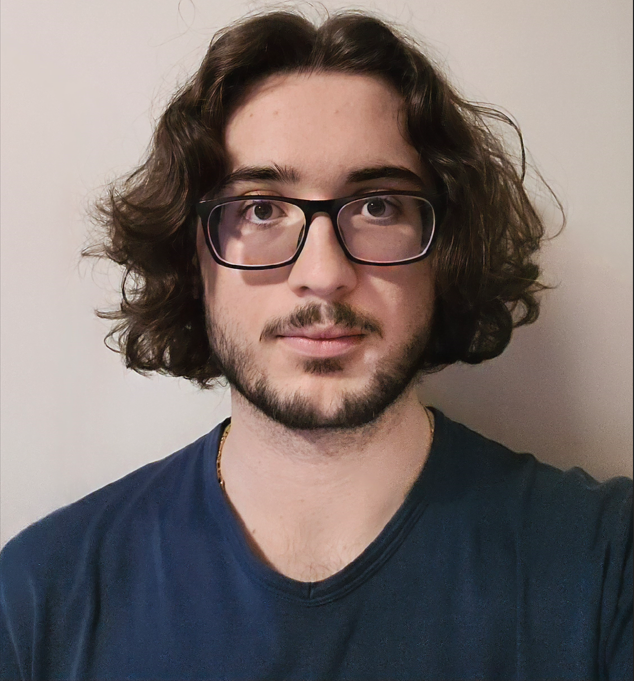
\includegraphics[width=1in,height=1.25in,clip,keepaspectratio]{imgs/andre.png}}]{André Filho}
  (M, 21) é um engenheiro de \textit{software} na Interlog Group, onde concentrou a sua experiência profissional no desenvolvimento \textit{web}. Licenciou-se em 2024 em Engenharia Informática pelo Instituto Politécnico de Leiria. Atualmente, frequenta o Mestrado em Cibersegurança e Informática Forense na mesma instituição, aprofundando os seus conhecimentos nesta área em crescimento.
\end{IEEEbiography}

\vfill

Vídeo da demonstração da componente prática: https://www.youtube.com/watch?v=nWVITOYAwYE.


Código-fonte da demonstração prática, localizado na diretoria assi-demo: https://github.com/ricardomlpereira/assi-project.

% You can push biographies down or up by placing
% a \vfill before or after them. The appropriate
% use of \vfill depends on what kind of text is
% on the last page and whether or not the columns
% are being equalized.

%\vfill

% Can be used to pull up biographies so that the bottom of the last one
% is flush with the other column.
%\enlargethispage{-5in}

% that's all folks
\end{document}

% bloatware

% An example of a floating figure using the graphicx package.
% Note that \label must occur AFTER (or within) \caption.
% For figures, \caption should occur after the \includegraphics.
% Note that IEEEtran v1.7 and later has special internal code that
% is designed to preserve the operation of \label within \caption
% even when the captionsoff option is in effect. However, because
% of issues like this, it may be the safest practice to put all your
% \label just after \caption rather than within \caption{}.
%
% Reminder: the "draftcls" or "draftclsnofoot", not "draft", class
% option should be used if it is desired that the figures are to be
% displayed while in draft mode.
%
%\begin{figure}[!t]
%\centering
%\includegraphics[width=2.5in]{myfigure}
% where an .eps filename suffix will be assumed under latex, 
% and a .pdf suffix will be assumed for pdflatex; or what has been declared
% via \DeclareGraphicsExtensions.
%\caption{Simulation results for the network.}
%\label{fig_sim}
%\end{figure}

% Note that the IEEE typically puts floats only at the top, even when this
% results in a large percentage of a column being occupied by floats.


% An example of a double column floating figure using two subfigures.
% (The subfig.sty package must be loaded for this to work.)
% The subfigure \label commands are set within each subfloat command,
% and the \label for the overall figure must come after \caption.
% \hfil is used as a separator to get equal spacing.
% Watch out that the combined width of all the subfigures on a 
% line do not exceed the text width or a line break will occur.
%
%\begin{figure*}[!t]
%\centering
%\subfloat[Case I]{\includegraphics[width=2.5in]{box}%
%\label{fig_first_case}}
%\hfil
%\subfloat[Case II]{\includegraphics[width=2.5in]{box}%
%\label{fig_second_case}}
%\caption{Simulation results for the network.}
%\label{fig_sim}
%\end{figure*}
%
% Note that often IEEE papers with subfigures do not employ subfigure
% captions (using the optional argument to \subfloat[]), but instead will
% reference/describe all of them (a), (b), etc., within the main caption.
% Be aware that for subfig.sty to generate the (a), (b), etc., subfigure
% labels, the optional argument to \subfloat must be present. If a
% subcaption is not desired, just leave its contents blank,
% e.g., \subfloat[].


% An example of a floating table. Note that, for IEEE style tables, the
% \caption command should come BEFORE the table and, given that table
% captions serve much like titles, are usually capitalized except for words
% such as a, an, and, as, at, but, by, for, in, nor, of, on, or, the, to
% and up, which are usually not capitalized unless they are the first or
% last word of the caption. Table text will default to \footnotesize as
% the IEEE normally uses this smaller font for tables.
% The \label must come after \caption as always.
%
%\begin{table}[!t]
%% increase table row spacing, adjust to taste
%\renewcommand{\arraystretch}{1.3}
% if using array.sty, it might be a good idea to tweak the value of
% \extrarowheight as needed to properly center the text within the cells
%\caption{An Example of a Table}
%\label{table_example}
%\centering
%% Some packages, such as MDW tools, offer better commands for making tables
%% than the plain LaTeX2e tabular which is used here.
%\begin{tabular}{|c||c|}
%\hline
%One & Two\\
%\hline
%Three & Four\\
%\hline
%\end{tabular}
%\end{table}


% Note that the IEEE does not put floats in the very first column
% - or typically anywhere on the first page for that matter. Also,
% in-text middle ("here") positioning is typically not used, but it
% is allowed and encouraged for Computer Society conferences (but
% not Computer Society journals). Most IEEE journals/conferences use
% top floats exclusively. 
% Note that, LaTeX2e, unlike IEEE journals/conferences, places
% footnotes above bottom floats. This can be corrected via the
% \fnbelowfloat command of the stfloats package.




% if have a single appendix:
%\appendix[Proof of the Zonklar Equations]
% or
%\appendix  % for no appendix heading
% do not use \section anymore after \appendix, only \section*
% is possibly needed

% use appendices with more than one appendix
% then use \section to start each appendix
% you must declare a \section before using any
% \subsection or using \label (\appendices by itself
% starts a section numbered zero.)
%


%\appendices
%\section{Proof of the First Zonklar Equation}
%Appendix one text goes here.

% you can choose not to have a title for an appendix
% if you want by leaving the argument blank
%\section{}
%Appendix two text goes here.



% trigger a \newpage just before the given reference
% number - used to balance the columns on the last page
% adjust value as needed - may need to be readjusted if
% the document is modified later
%\IEEEtriggeratref{8}
% The "triggered" command can be changed if desired:
%\IEEEtriggercmd{\enlargethispage{-5in}}

